\documentclass{article}
\PassOptionsToPackage{numbers}{natbib}
\usepackage[preprint]{neurips_2024}

\usepackage[utf8]{inputenc}
\usepackage[T1]{fontenc}
\usepackage{hyperref}
\usepackage{url}
\usepackage{booktabs}
\usepackage{amsfonts}
\usepackage{microtype}
\usepackage{graphicx}
\usepackage{algorithm}
\usepackage{algorithmic}
\usepackage{amsmath,amssymb}
\usepackage{multirow}
\usepackage{xcolor}

% --- Work-in-progress review annotations (remove for camera-ready) ---
\newcommand{\reviewnote}[1]{%
  \par\smallskip\noindent
  \fcolorbox{orange!80!black}{orange!10}{%
    \parbox{\dimexpr\linewidth-2\fboxsep-2\fboxrule\relax}{%
      \footnotesize\textbf{\textcolor{orange!70!black}{[Review flag --- known open issue, WIP]:}}~#1}}%
  \par\smallskip}

\title{xskill: Team-Level Skill Distillation, Sharing,\\ and Evolution for Coding Agents}

\author{
  SkillNerds Team \\
  \texttt{https://github.com/SkillNerds/xskill}
}

\begin{document}

\maketitle

\begin{abstract}
Coding agents increasingly rely on \emph{skills}---reusable markdown documents that encode procedural knowledge for recurring tasks. In team settings, skills learned by one developer remain trapped in individual session histories. We present \textbf{xskill}, an open-source framework that operates as a management layer above coding-agent runtimes to automatically distill skills from real user trajectories, share them across a team, and evolve them through data-driven canary deployment. xskill's three-agent pipeline (TaskAgent, TaskClusterAgent, SkillEditAgent) decomposes trajectories into atomic task segments, clusters them into skill candidates with cumulative evidence thresholds, and produces versioned SKILL.md artifacts via git commits. A canary evaluation protocol---drawing on established online controlled experiment methodology---routes a subset of users to staging skill versions and compares behavioral UX scores against the main branch, promoting or freezing candidates based on statistical evidence. A cross-sectional source-code-level survey of 11 trajectory-to-skill systems reveals that controlled A/B comparison of skill versions is essentially absent---only concurrent work (SkillClaw) performs any such comparison, and it does so offline on fixed validation scenarios with machine reward signals rather than online on live traffic---and that skill quality across all systems is ceiling-bounded by the authoring LLM's capability. We provide a deployment scenario analysis using real skill inventory data (139 loaded skills whose 26{,}448-character listing exceeds the agent's listing budget $\approx$3.3$\times$) and formalize the UX scoring function and canary statistical protocol. xskill brings together asynchronous cross-agent trajectory collection across five ecosystems, cumulative-evidence skill production, and multi-runtime skill distribution, and---to our knowledge---is the first to evaluate skill evolution via \emph{online behavioral-UX canary} on live team traffic.
\end{abstract}

\reviewnote{\textbf{This is a work-in-progress preprint.} An internal three-reviewer pass flagged the following open issues, which we acknowledge and will address with experiments in a future revision: (i)~\emph{no controlled empirical evaluation yet}---the worked example, throughput, and convergence numbers are illustrative/estimated, not measured (a real team deployment is the central planned experiment); (ii)~the UX scoring function and its constants are unvalidated defaults pending calibration against ground-truth satisfaction; (iii)~the canary's statistical protocol needs user-clustered / sequential / FDR-controlled testing before promotion decisions can be called sound (\S\ref{sec:canary}); (iv)~whether online behavioral evaluation reaches \emph{materially different} decisions than offline scenario A-B (vs.\ concurrent SkillClaw) is not yet empirically isolated. These are deliberately surfaced early; the design and claims are written to be defensible without these experiments, which remain future work.}

%============================================================================
\section{Introduction}
\label{sec:intro}
%============================================================================

The rise of agentic coding assistants---Claude Code~\citep{anthropic2025claude}, Codex~\citep{openai2025codex}, OpenCode~\citep{sst2025opencode}, and others---has transformed software development workflows. These agents leverage \emph{skills}: reusable, markdown-formatted procedural documents (typically named \texttt{SKILL.md}) that encode domain-specific knowledge, best practices, and step-by-step instructions for recurring tasks. The concept parallels long-standing observations in organizational knowledge management~\citep{nonaka1995knowledge}: valuable procedural knowledge is generated through practice but easily lost without systematic capture and distribution mechanisms.

In team settings, the skill problem compounds. Developer~A spends an afternoon teaching her agent a deployment workflow; Developer~B, facing the same task, starts from scratch. The knowledge is trapped in individual session histories. Even when a workflow is manually documented as a skill, there is no mechanism to:
\begin{itemize}
    \item \textbf{Automatically distill} successful agent trajectories into reusable skills;
    \item \textbf{Share and distribute} skills across team members with appropriate sanitization;
    \item \textbf{Evolve} skills based on real usage data, retiring those that degrade and promoting those that help.
\end{itemize}

\begin{figure*}[t]
\centering
\includegraphics[width=0.92\textwidth]{figures/fig_teaser.png}
\caption{Conceptual overview of xskill's skill distillation cycle. Developers' coding sessions (left) produce trajectory streams that flow into a central distillation hub (center), which extracts and refines reusable skill documents distributed back to the team (right).}
\label{fig:teaser}
\end{figure*}

\begin{figure}[t]
\centering
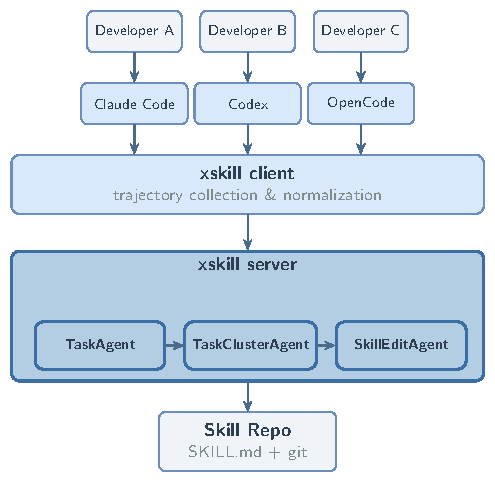
\includegraphics[width=0.52\textwidth]{figures/fig1_overview.pdf}
\caption{\textbf{xskill system overview.} Developers use their preferred coding agents. The xskill client daemon watches trajectory directories and uploads sanitized deltas to the central server. The server's three-agent pipeline decomposes trajectories into atomic tasks, clusters them into skill candidates, and produces versioned SKILL.md artifacts via git commits. Evolved skills are synced back to each developer's agent runtime.}
\label{fig:overview}
\end{figure}

We present \textbf{xskill}, an open-source system that addresses all three challenges. xskill operates as a \emph{management layer} above existing coding-agent runtimes (Figure~\ref{fig:overview}). It does not replace any agent's skill loader; instead, it shapes what those loaders read from disk. The key insight is that the \emph{lifecycle} of a skill---creation, evaluation, evolution, retirement---is orthogonal to the \emph{runtime} that loads and injects skills into agent prompts, and should therefore be managed by a dedicated system.

Our contributions are:
\begin{enumerate}
    \item A \textbf{cross-agent trajectory collection} architecture supporting 5 coding-agent ecosystems through a unified normalizer interface (\S\ref{sec:collection}).
    \item A \textbf{three-agent pipeline} with cumulative evidence thresholds for automatic skill distillation, formalized as Algorithm~\ref{alg:pipeline} (\S\ref{sec:pipeline}).
    \item A \textbf{canary evaluation protocol} using git branching, behavioral UX scoring, and statistical significance testing---to our knowledge the first \emph{online, live-traffic} such mechanism in the trajectory-to-skill literature, formalized as Algorithm~\ref{alg:canary} (\S\ref{sec:canary}).
    \item A \textbf{comprehensive source-code-level survey} of 11 trajectory-to-skill systems across 5 design dimensions, providing the first systematic comparison for this emerging field (\S\ref{sec:related}, \S\ref{sec:dimensions}).
    \item A \textbf{deployment scenario analysis} with real skill inventory data and an \emph{illustrative} worked example walking through the full skill lifecycle (\S\ref{sec:evaluation}). We are explicit that this is a design/scenario analysis, not a controlled empirical evaluation (\S\ref{sec:discussion}).
\end{enumerate}

%============================================================================
\section{Related Work}
\label{sec:related}
%============================================================================

We surveyed 11 systems that convert agent trajectories or experiences into reusable procedural knowledge. Table~\ref{tab:landscape} presents the landscape overview. All assessments were verified against source code (with path:line citations released alongside the open-source code) rather than documentation claims alone. Below we discuss the most instructive comparisons and connect xskill to the broader research landscape.

\begin{table}[t]
\centering
\caption{\textbf{Landscape of trajectory-to-skill systems.} Columns indicate whether the system produces SKILL.md files, supports online (per-turn) triggering, implements deduplication, performs canary/A-B evaluation, and targets production coding-agent deployment. The 11 rows above the rule are the surveyed systems; SkillClaw ($^\dagger$) is concurrent work shown for comparison and is \emph{not} counted among the 11. xskill (below the rule) is our system.}
\label{tab:landscape}
\small
\begin{tabular}{@{}lccccc@{}}
\toprule
\textbf{System} & \textbf{SKILL.md} & \textbf{Online} & \textbf{Dedup} & \textbf{Canary} & \textbf{Production} \\
\midrule
OpenSpace      & \checkmark & \checkmark & \checkmark & $\times$ & \checkmark \\
EvoSkill       & \checkmark & $\times$   & $\times$   & $\times$ & \checkmark \\
AutoSkill      & \checkmark & \checkmark & \checkmark & $\times$ & \checkmark \\
Hermes         & \checkmark & $\times$   & $\times$   & $\times$ & $\times$ \\
GEPA-gskill    & \checkmark & $\times$   & $\times$   & $\times$ & $\times$ \\
Trace2Skill    & $\times$   & $\times$   & $\times$   & $\times$ & $\times$ \\
AgentEvolver   & $\times$   & $\times$   & $\times$   & $\times$ & $\times$ \\
MemSkill       & $\times$   & $\times$   & $\times$   & $\times$ & $\times$ \\
EvoAgentX      & $\times$   & $\times$   & $\times$   & $\times$ & $\times$ \\
SE-Agent       & $\times$   & $\times$   & $\times$   & $\times$ & $\times$ \\
SkillRL        & $\times$   & $\times$   & $\times$   & $\times$ & $\times$ \\
SkillClaw      & \checkmark & $\times$   & $\times$   & \checkmark$^\dagger$ & \checkmark \\
\midrule
\textbf{xskill} & \checkmark & \checkmark & \checkmark & \checkmark & \checkmark \\
\bottomrule
\end{tabular}

{\footnotesize $^\dagger$SkillClaw (concurrent work) performs \emph{offline} validation-scenario A-B (candidate vs.\ current skill on idle clients), not online canary on live production traffic.}
\end{table}

\subsection{Skill-as-SKILL.md Systems}

\textbf{OpenSpace}~\citep{hku2025openspace} is the closest system to xskill in scope. It maintains an evolving skill library via an MCP server, with three evolution triggers (per-task analysis, tool-degradation events, and periodic counters) feeding into a 3$\times$3 evolution type matrix (FIX / DERIVED / CAPTURED). However, OpenSpace wraps skill execution inside its own sub-agent---meaning the host agent's harness (e.g., \texttt{CLAUDE.md} rules) does not apply during skill-enhanced execution, a fundamental isolation problem for production use. OpenSpace evaluates skills via success/failure counts and LLM judgments, but never compares skill versions against each other in a controlled setting.

\textbf{EvoSkill}~\citep{sentient2025evoskill} uses git branches as program versions and Pareto frontiers for selection, offering the cleanest version-control story among all surveyed systems. However, it requires offline batch execution and does not support real-time trajectory collection.

\textbf{AutoSkill}~\citep{ecnu2025autoskill} is the only system besides xskill that achieves per-turn asynchronous skill extraction during live chat. Its multi-stage deduplication pipeline (identity hash $\to$ semantic$+$BM25 $\to$ LLM judge; six stages in full, Table~\ref{tab:dedup}) is the most sophisticated deduplication mechanism we found. AutoSkill also provides the only per-turn usage tracking via an LLM judge that labels each injected skill as \texttt{relevant}/\texttt{used}, but this measures skill \emph{selection} quality, not downstream user experience.

\textbf{Trace2Skill}~\citep{alibaba2025trace2skill} proposes a MapReduce-style patch merging approach and demonstrates that machine-generated skills can outperform human-written ones on SpreadsheetBench. Its key finding---cross-model skill transfer is viable---supports xskill's design of centralized skill production serving heterogeneous client runtimes.

\textbf{SkillClaw}~\citep{amapml2026skillclaw}, concurrent with our work, is the most similar system in goal: it performs collective, cross-user skill evolution for coding agents, capturing real sessions and evolving a shared library of SKILL.md bundles. Architecturally it differs from xskill in three notable ways. First, it integrates via a \emph{man-in-the-middle proxy} that intercepts OpenAI/Anthropic API calls and splices retrieved skills into the system prompt, rather than mounting each runtime's native skills directory; this is runtime-agnostic but decoupled from the host harness's native loader. Second, its evolution operates at \emph{whole-session} granularity driven by a single agentic evolver (improve / optimize-description / create / skip), in contrast to xskill's sub-trajectory decomposition and three-agent division of labor. Third---and most relevant to evaluation---SkillClaw \emph{does} validate candidate skills before deployment, but via \emph{offline} A-B on fixed validation scenarios run in idle client environments, scored by process/outcome reward models, with all-or-nothing promotion rather than gradual rollout. xskill instead routes live team traffic to staging versions and compares behavioral UX scores under a statistical promotion protocol (\S\ref{sec:canary}). The two regimes are complementary: SkillClaw's is reproducible and pre-deployment; xskill's measures realized user benefit on production traffic. We are candid that whether the two regimes reach \emph{materially different} promote/freeze decisions on the same candidates is an open empirical question we have not yet resolved; establishing that online behavioral evaluation changes outcomes (not merely the methodology) is the key experiment this design motivates.

\subsection{Non-SKILL.md Systems and Broader Context}

Several systems use alternative skill representations: \textbf{MemSkill}~\citep{memskill2025} trains PPO controllers over operation banks; \textbf{EvoAgentX}~\citep{evoagentx2025} evolves workflow code; \textbf{SE-Agent}~\citep{seagent2025} replaces per-instance system prompts; \textbf{SkillRL}~\citep{skillrl2025} trains RL agents with JSON skill records; and \textbf{AgentEvolver}~\citep{agentevolver2025} delegates to an external ReMe memory service. These target RL training loops rather than production coding-agent deployments. \textbf{GEPA}~\citep{gepa2025} introduces system-aware three-way merge by common ancestor, analogous to git's merge algorithm applied to prompt evolution.

xskill also connects to the broader literature on agent self-improvement. \textbf{Voyager}~\citep{wang2023voyager} pioneered the concept of an automatically growing skill library for embodied agents in Minecraft, demonstrating that LLM-authored programs can compose into increasingly complex behaviors. \textbf{Reflexion}~\citep{shinn2023reflexion} showed that agents can improve from trajectory-level verbal feedback, an insight that motivates xskill's use of trajectory-derived UX signals rather than outcome-only rewards. The prompt optimization literature---including DSPy~\citep{khattab2023dspy} and OPRO~\citep{yang2024opro}---has established that LLM-generated textual artifacts (prompts, demonstrations) can be systematically optimized; xskill extends this paradigm from prompt tuning to full skill document evolution in multi-agent team settings.

\subsection{The Evaluation Gap: Proxy Metrics and the Absence of Online Canary}

Among the 11 surveyed systems, \emph{none} implements controlled A/B comparison of skill versions. The lone exception in the broader landscape is the concurrent SkillClaw~\citep{amapml2026skillclaw}, which validates candidate skills before deployment---but \emph{offline}, on fixed validation scenarios run in idle client environments and scored by process/outcome reward models, with all-or-nothing promotion. Most surveyed systems instead evaluate skills via offline benchmarks (EvoSkill, GEPA, MemSkill) or LLM-as-judge on the skill text itself (OpenSpace). Only AutoSkill tracks per-turn \texttt{relevant/used} judgments, but this measures skill selection quality, not downstream user experience. What remains absent across \emph{all} of these systems is \emph{online} controlled comparison on live traffic with a direct user-experience signal: skill evolution is driven by proxy metrics or offline pre-deployment checks rather than by realized user benefit in production---a gap xskill explicitly addresses.

This gap is surprising given the mature literature on online controlled experiments~\citep{kohavi2013online, kohavi2020trustworthy}, where A/B testing has been standard practice in web systems for over a decade. The canary evaluation protocol (\S\ref{sec:canary}) adapts these principles to the skill evaluation setting, where sample sizes are smaller (team-level rather than web-scale) but the evaluation target (a versioned SKILL.md document) is well-suited to branch-based experimental design.


%============================================================================
\section{System Architecture}
\label{sec:architecture}
%============================================================================

xskill consists of two components: a \textbf{client daemon} running on each developer's machine, and a \textbf{central server} that hosts the three-agent pipeline and the skill repository.

\subsection{Cross-Agent Trajectory Collection}
\label{sec:collection}

\begin{figure}[t]
\centering
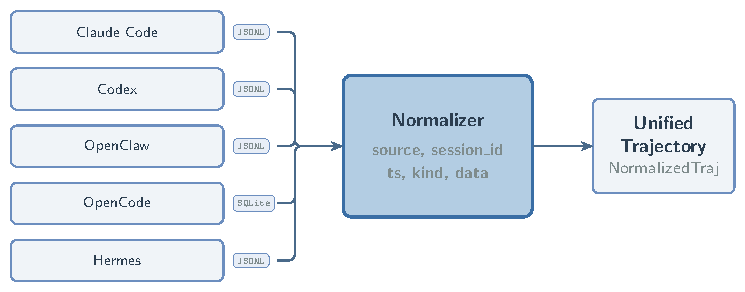
\includegraphics[width=0.95\textwidth]{figures/fig2_collection.pdf}
\caption{\textbf{Cross-agent trajectory collection.} Each coding agent writes trajectories in its native format. The xskill client runs per-agent adapters that normalize events into a unified schema. Four of five agents use appendable JSONL, enabling efficient \texttt{inotify}/\texttt{tail} collection; OpenCode's SQLite database requires polling.}
\label{fig:collection}
\end{figure}

A key design decision is that xskill does \emph{not} require agents to push trajectories; instead, the client daemon \emph{pulls} from known filesystem locations (Figure~\ref{fig:collection}). This zero-configuration approach works because all five supported agents write trajectories to predictable, stable paths (detailed in Appendix~\ref{app:paths}).

Each trajectory event is normalized into a \texttt{TrajectoryEvent} schema with fields: \texttt{source} (agent identifier), \texttt{session\_id}, \texttt{ts} (ISO~8601), \texttt{kind} $\in$ \{user\_msg, assistant\_msg, tool\_call, tool\_result, session\_start, session\_end, compact\}, and \texttt{data} (native payload preserved for replay). The watcher scans registered directories every 30 seconds; new or appended content triggers the three-agent pipeline.

\paragraph{Sanitization.} Before upload, the client applies secret-pattern redaction (API keys, tokens, credentials) using a configurable regex set. This is critical for team-shared trajectories: our ecosystem survey found that only 3 of 11 systems (Hermes, AutoSkill, OpenSpace) implement any form of secret redaction, and none addresses the subtler question of implicit intellectual property in trajectories.

\subsection{Three-Agent Pipeline}
\label{sec:pipeline}

\begin{figure}[t]
\centering
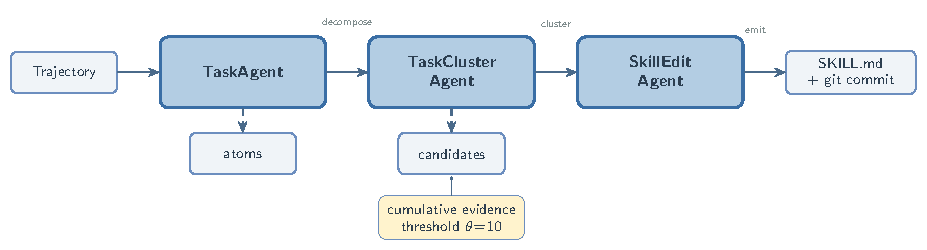
\includegraphics[width=\textwidth]{figures/fig3_pipeline.pdf}
\caption{Conceptual illustration of the three-agent pipeline. Raw conversation trajectories (left) are segmented into atomic tasks, routed into skill-specific categories, and synthesized into polished SKILL.md documents with git version control (right). The formal pipeline is specified in Algorithm~\ref{alg:pipeline}.}
\label{fig:pipeline}
\end{figure}

The server processes normalized trajectories through three specialized agents (Figure~\ref{fig:pipeline}). Algorithm~\ref{alg:pipeline} formalizes the complete flow.

\begin{algorithm}[t]
\caption{Three-Agent Skill Distillation Pipeline}
\label{alg:pipeline}
\begin{algorithmic}[1]
\REQUIRE Trajectory delta $\delta$, skill catalog $\mathcal{C}$, threshold $\theta = 10$
\ENSURE Updated skill repository
\STATE \textbf{Stage 1: TaskAgent} --- Decompose $\delta$ into AtomTasks
\STATE $\mathcal{A} \leftarrow \texttt{TaskAgent.decompose}(\delta)$ \COMMENT{Segment by semantic boundaries}
\FOR{each atom $a \in \mathcal{A}$}
    \STATE Assign $a.\mathrm{ux\_score} \leftarrow f_{\mathrm{UX}}(a)$ \COMMENT{Behavioral UX scoring (Eq.~\ref{eq:ux})}
    \STATE Record $a.\mathrm{intent}, a.\mathrm{tags}, a.\mathrm{used\_skills}$
\ENDFOR
\STATE
\STATE \textbf{Stage 2: TaskClusterAgent} --- Route atoms to skills
\FOR{each atom $a \in \mathcal{A}$}
    \STATE $(\mathrm{action}, \mathrm{skill}, w) \leftarrow \texttt{TCA.route}(a, \mathcal{C})$
    \IF{$\mathrm{action} = \texttt{CREATE}$}
        \STATE Initialize new skill folder in ``baby'' state with $a$ as first evidence
        \STATE $\mathcal{C} \leftarrow \mathcal{C} \cup \{\mathrm{skill}\}$
    \ELSIF{$\mathrm{action} = \texttt{ROUTE}$}
        \STATE Append $(a, w)$ to $\mathrm{skill}$.\texttt{candidates.yml}
    \ELSIF{$\mathrm{action} = \texttt{RECLASSIFY}$}
        \STATE Move $a$ from current skill to better-fit target
    \ENDIF
\ENDFOR
\STATE
\STATE \textbf{Stage 3: SkillEditAgent} --- Produce or update skills
\FOR{each skill $s \in \mathcal{C}$}
    \IF{$\sum_{(a,w) \in s.\mathrm{candidates}} w \geq \theta$ \AND canary guards pass}
        \STATE $\texttt{SKILL.md} \leftarrow \texttt{SEA.generate}(s.\mathrm{candidates}, s.\mathrm{existing\_body})$
        \IF{$s.\mathrm{branch} = \texttt{baby}$}
            \STATE \texttt{git commit} to \texttt{main} \COMMENT{First public version}
        \ELSE
            \STATE \texttt{git commit} to \texttt{staging} \COMMENT{Canary candidate}
        \ENDIF
    \ENDIF
\ENDFOR
\end{algorithmic}
\end{algorithm}

\subsubsection{TaskAgent: Trajectory Decomposition}

Raw trajectories are multi-topic conversations that may span hours. The TaskAgent segments each trajectory into \textbf{AtomTasks}---coherent units representing a single user intent (e.g., ``deploy FastAPI to port 1717'' or ``fix the SQLite migration''). Each AtomTask records: a unique \texttt{atom\_id}, semantic metadata (\texttt{intent}, \texttt{summary}, \texttt{tags}), provenance (\texttt{offset\_start}, \texttt{offset\_end}), a \texttt{ux\_score} used in canary evaluation, and linked-list pointers to neighboring atoms for context recovery. The full AtomTask schema is given in Appendix~\ref{app:atomtask}.

\paragraph{UX Scoring Function.} The UX score (written $f_{\mathrm{UX}}$ in Algorithm~\ref{alg:pipeline}, $s(a)$ here) is the central evaluation signal in xskill's canary protocol. Unlike LLM-as-judge approaches used by OpenSpace and AutoSkill, the UX score is derived from \emph{observable behavioral signals}. Formally, given an AtomTask $a$, the score is:
\begin{equation}
\label{eq:ux}
s(a) = w_1 \cdot \mathrm{completion}(a) + w_2 \cdot \left(1 - \min\!\left(\frac{\mathrm{corrections}(a)}{3},\; 1\right)\right) + w_3 \cdot \mathrm{attribution}(a)
\end{equation}
where:
\begin{itemize}
    \item $\mathrm{completion}(a) \in \{0, 1\}$: whether the atom's intent was fulfilled, detected by the presence of a natural topic transition vs.\ session abandonment or explicit user cancellation.
    \item $\mathrm{corrections}(a) \in \mathbb{Z}_{\geq 0}$: the number of user corrections following the agent's output, detected by user messages containing negation, redirection, or explicit ``no/wrong/redo'' patterns within the atom boundary. The score saturates at 3 corrections (any further corrections yield the same minimum contribution).
    \item $\mathrm{attribution}(a) \in \{0, 1\}$: whether a skill was self-reported as used during this atom (from the \texttt{used\_skills} field). This signal enables per-skill UX attribution.
    \item Default weights: $w_1 = 5, w_2 = 3, w_3 = 2$, yielding $s \in [0, 10]$.
\end{itemize}

The intended distinction from LLM-as-judge evaluation~\citep{zheng2024judging} is one of \emph{target}: rather than asking a model to rate output \emph{quality} directly (which exhibits a documented self-preference bias), the TaskAgent extracts \emph{observable} indicators (a topic transition, a ``no/wrong/redo'' user message). We are careful not to overstate this: signal extraction is still LLM-mediated, so it inherits classification noise---the $\mathrm{completion}$ and $\mathrm{corrections}$ detectors are heuristics whose error rates we have not yet measured (e.g., a follow-up question may be misread as a correction, \S\ref{sec:discussion})---and the attribution term depends on agents self-reporting \texttt{used\_skills}, which not all runtimes do consistently. The weights ($w_1{=}5,w_2{=}3,w_3{=}2$) and the other constants in this protocol ($\theta{=}10$, correction saturation at 3, $n_{\min}{=}20$, $\rho{\le}0.5$, $\Delta_{\min}{=}0.5$, $T_{\max}{=}30$d) are \emph{defaults}, not tuned or validated against an independent satisfaction measure; calibrating them and validating that $s(a)$ tracks ground-truth user benefit is important future work. The claim here is modest---that observable signals are a reasonable, less self-referential basis for canary comparison than self-rating---not that $s(a)$ is a validated measure of skill quality.

\subsubsection{TaskClusterAgent: Skill Routing}

Each AtomTask triggers a TaskClusterAgent (TCA) invocation. The TCA receives the atom plus the top-$k$ existing skills retrieved from the catalog by embedding similarity (each as name + truncated description) and makes one of three decisions: (1)~\textbf{Route to existing skill}: append the atom to the skill's \texttt{.candidates.yml} with a \texttt{weightscore} ($0$--$10$) reflecting the atom's relevance; (2)~\textbf{Create new skill}: initialize a new skill folder in ``baby'' state with the atom as first evidence; (3)~\textbf{Reclassify}: move an atom from one skill to another if the TCA determines a better fit.

The TCA's routing is LLM-based but constrained by the existing catalog structure, preventing unbounded skill proliferation while allowing organic growth. This positions xskill's deduplication at a moderate complexity level: more sophisticated than systems with zero deduplication (Hermes, SE-Agent, EvoAgentX) or simple string matching (SkillRL), but deliberately less complex than AutoSkill's six-layer sandwich. The rationale is that catalog-aware routing combined with cumulative evidence provides sufficient quality control without the engineering complexity of multi-stage dedup pipelines.

\subsubsection{SkillEditAgent: Skill Production}

When a skill's \texttt{.candidates.yml} accumulates a cumulative \texttt{weightscore} $\geq \theta$ (default $\theta = 10$), the SkillEditAgent (SEA) fires. The threshold value was chosen empirically: $\theta = 10$ requires contributions from at least 2--3 distinct trajectories at moderate relevance scores, ensuring that no skill is produced from a single interaction. The SEA reads all candidate atoms and produces or updates the skill's \texttt{SKILL.md}.

The SEA's commit behavior depends on branch state: (1)~\textbf{Baby branch $\to$ main}: first public version of a new skill; (2)~\textbf{Main branch $\to$ staging}: creates a canary candidate for A/B comparison. This branching model ensures that skill updates are never applied directly to main without canary evaluation.

\subsection{Canary Evaluation Protocol}
\label{sec:canary}

\begin{figure}[t]
\centering
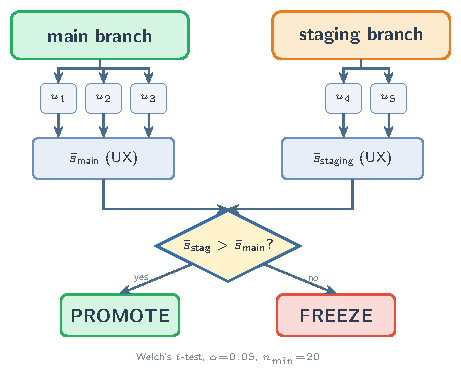
\includegraphics[width=0.5\textwidth]{figures/fig4_canary.pdf}
\caption{\textbf{Canary evaluation protocol.} When the SkillEditAgent produces an updated skill, it commits to a staging branch. A subset of users receives the staging version while the majority continues on main. UX scores from AtomTasks using each branch are aggregated; the staging branch is promoted only if statistically superior.}
\label{fig:canary}
\end{figure}

The canary protocol (Figure~\ref{fig:canary}) is xskill's primary quality gate, drawing on the methodology of online controlled experiments~\citep{kohavi2013online, kohavi2020trustworthy} adapted for the team-level skill evaluation setting. Algorithm~\ref{alg:canary} formalizes the procedure.

\begin{algorithm}[t]
\caption{Canary Evaluation Protocol}
\label{alg:canary}
\begin{algorithmic}[1]
\REQUIRE Skill $s$ with new staging commit, user set $U$, routing fraction $\rho \in (0, 0.5]$, minimum samples $n_{\min} = 20$, significance level $\alpha = 0.05$, timeout $T_{\max}$ days
\ENSURE Decision $\in \{\texttt{PROMOTE}, \texttt{FREEZE}, \texttt{TIMEOUT}\}$
\STATE \textbf{Guard conditions:}
\STATE \quad Assert no active staging branch for $s$ (one canary at a time; new candidates queue)
\STATE \quad Assert $\geq 1$ real $\mathrm{side}=\mathrm{main}$ UX score exists (baseline established)
\STATE
\STATE \textbf{User routing:}
\STATE Route $\lceil \rho |U| \rceil$ users to staging; remainder to main
\STATE
\STATE \textbf{Score collection:}
\WHILE{$|S_{\mathrm{main}}| < n_{\min}$ \OR $|S_{\mathrm{staging}}| < n_{\min}$}
    \IF{elapsed $> T_{\max}$}
        \RETURN \texttt{TIMEOUT} (freeze staging, retain for audit)
    \ENDIF
    \STATE Collect UX scores $s_i$ from AtomTasks using skill $s$
    \STATE Attribute each $s_i$ to $S_{\mathrm{main}}$ or $S_{\mathrm{staging}}$ based on user's branch
\ENDWHILE
\STATE
\STATE \textbf{Statistical comparison:}
\STATE Compute $\bar{s}_{\mathrm{main}}, \bar{s}_{\mathrm{staging}}, \sigma_{\mathrm{main}}, \sigma_{\mathrm{staging}}$
\STATE Perform one-sided Welch's $t$-test: $H_0\!: \mu_{\mathrm{staging}} \leq \mu_{\mathrm{main}}$
\IF{$p < \alpha$ \AND $\bar{s}_{\mathrm{staging}} > \bar{s}_{\mathrm{main}}$}
    \STATE Merge staging $\to$ main; \RETURN \texttt{PROMOTE}
\ELSE
    \STATE Freeze staging (retain for audit, hide from distribution); \RETURN \texttt{FREEZE}
\ENDIF
\end{algorithmic}
\end{algorithm}

Key design decisions in the canary protocol:

\paragraph{Single active canary per skill.} At most one staging branch exists for any given skill at any time. If the SkillEditAgent produces a new candidate while a canary is active, the candidate is queued rather than overwriting the current experiment. This prevents evaluation contamination from concurrent canaries---a principle directly borrowed from controlled experiment methodology~\citep{kohavi2020trustworthy}.

\paragraph{Behavioral UX scores, not LLM self-evaluation.} The UX score (Eq.~\ref{eq:ux}) is derived from observable signals in the trajectory, not from asking an LLM to rate its own output. This distinguishes xskill from the LLM-as-judge approaches used by OpenSpace (success/failure counts via LLM) and AutoSkill (LLM-labeled relevant/used). While behavioral signals are noisier than LLM judgments, they avoid the systematic upward bias documented in MT-Bench evaluations~\citep{zheng2024judging}.

\paragraph{Statistical protocol.} The minimum sample size ($n_{\min} = 20$ per branch) and significance level ($\alpha = 0.05$, one-sided Welch's $t$-test) reflect the team-level deployment context where sample sizes are inherently smaller than web-scale A/B tests. For teams with fewer than 10 active developers, the timeout mechanism ($T_{\max}$, default 30 days) ensures that experiments do not run indefinitely. When traffic is insufficient for statistical power, xskill falls back to a simple mean comparison with a required minimum effect size ($\Delta_{\min} = 0.5$ points on the 0--10 scale), trading statistical rigor for practical convergence.

\paragraph{Threats to statistical validity (and planned mitigations).} We make the limitations of the current test explicit rather than overstate its rigor. (1)~\textbf{Non-independence / pseudo-replication.} AtomTask UX scores cluster within developers and within sessions, so the effective sample size is closer to the number of \emph{developers} than the number of atoms; a per-atom Welch's $t$-test therefore overstates power for the 5--10-person teams we target. A user-clustered (mixed-effects) or permutation test over users is the correct analysis and is planned. (2)~\textbf{Optional stopping.} Algorithm~\ref{alg:canary} collects until $n_{\min}$ and then tests once, which is safe, but any interim inspection would inflate Type-I error; a sequential test (e.g., always-valid $p$-values / mSPRT~\citep{kohavi2020trustworthy}) is the principled replacement. (3)~\textbf{Multiple comparisons.} Running an independent $\alpha=0.05$ test per skill across a large catalog (139 in \S\ref{sec:evaluation}) inflates family-wise false promotions; false-discovery-rate control across concurrent canaries is needed at scale. (4)~\textbf{Non-normal, bounded scores.} UX scores are bounded and discrete-ish, so a rank-based or permutation test is more appropriate than Welch's $t$ at small $n$. (5)~The low-traffic $\Delta_{\min}$ fallback has \emph{no} Type-I guarantee and, given realistic per-branch sample rates, may be the regime small teams most often hit; we report this honestly as a heuristic, not a test. These are design limitations of the present protocol, not of the canary concept; the git-branch mechanism is agnostic to which test sits on top.

\reviewnote{Flagged by all three reviewers. The upgrade to user-clustered / sequential / FDR-controlled testing, and a measurement of how often deployments hit the underpowered fallback, are planned with the deployment study.}

\subsection{Cross-Agent Skill Distribution}
\label{sec:distribution}

A critical finding from our ecosystem survey is that \textbf{SKILL.md with YAML frontmatter is the de facto cross-agent standard}. Five of the eleven surveyed systems produce this format, and all five supported agent runtimes parse it. xskill exploits this convergence: two filesystem paths---\texttt{\~{}/.claude/skills/} and \texttt{\~{}/.agents/skills/}---cover 4 of 5 ecosystems; only Hermes requires a dedicated \texttt{\~{}/.hermes/skills/} path.

The frontmatter uses a compatible superset where private fields (e.g., \texttt{metadata.hermes.tags}, \texttt{metadata.openclaw.emoji}) are silently ignored by non-target runtimes---all five do YAML-tolerant parsing---so a single artifact serves all ecosystems. Full distribution path details are in Appendix~\ref{app:distribution}.

%============================================================================
\section{Design Dimensions: A Comparative Analysis}
\label{sec:dimensions}
%============================================================================

Our survey organizes the trajectory-to-skill landscape into five dimensions. We present key findings per dimension, drawing implications for system design and positioning xskill's choices.

\subsection{Trigger Mechanism}

\begin{table}[t]
\centering
\caption{\textbf{Trigger mechanisms across 11 systems + xskill.} Nine of eleven systems use offline batch or counter-based triggers. Only OpenSpace and AutoSkill achieve user-transparent, per-turn triggering.}
\label{tab:trigger}
\small
\begin{tabular}{@{}lcccl@{}}
\toprule
\textbf{System} & \textbf{Async} & \textbf{Per-turn} & \textbf{Transparent} & \textbf{Mechanism} \\
\midrule
Hermes         & -- & -- & -- & Offline CLI \\
OpenSpace      & \checkmark & \checkmark & \checkmark & Hook + counter + event \\
EvoSkill       & -- & -- & -- & Offline batch \\
AutoSkill      & \checkmark & \checkmark & \checkmark & Per-turn + background thread \\
Trace2Skill    & -- & -- & -- & Offline patch merge \\
AgentEvolver   & -- & -- & -- & Counter in RL loop \\
MemSkill       & -- & -- & -- & Counter in RL loop \\
EvoAgentX      & -- & -- & -- & Offline batch loop \\
SE-Agent       & -- & -- & -- & Offline iteration \\
SkillRL        & -- & -- & -- & Counter + success gate \\
GEPA           & -- & -- & -- & Offline batch \\
\midrule
\textbf{xskill} & \checkmark & \checkmark & \checkmark & 30s watcher + per-atom async \\
\bottomrule
\end{tabular}
\end{table}

Nine of eleven systems use offline batch or counter-based triggers (Table~\ref{tab:trigger}). Only OpenSpace and AutoSkill achieve user-transparent, per-turn triggering. This indicates that the research community still largely treats trajectory-to-skill as an offline training concern; the engineering costs of async/concurrent/performance-aware real-time distillation have not been widely addressed. xskill adopts a 30-second polling watcher with per-atom asynchronous processing, achieving transparency without requiring hook registration in the host agent.

\subsection{Skill Production: LLM-as-Author is Universal}

All 11 systems use LLM-as-author for skill text generation---no system attempts rule-based, template, or AST-based production. This universality has a critical implication: \textbf{skill quality is ceiling-bounded by the authoring LLM's capability}. A skill can only be as good as the model that writes it, regardless of how many trajectories inform the generation.

xskill partially mitigates this ceiling through cumulative evidence: rather than generating a skill from a single trajectory (as OpenSpace, AutoSkill, and SE-Agent can), the SkillEditAgent waits for multiple weighted atoms to accumulate, providing richer context to the authoring LLM. This does not raise the ceiling, but it helps the LLM approach it more reliably.

\subsection{Deduplication and Merging}

\begin{table}[t]
\centering
\caption{\textbf{Deduplication maturity spectrum.} Systems range from zero deduplication to AutoSkill's six-layer sandwich. xskill occupies a moderate position with catalog-aware LLM routing.}
\label{tab:dedup}
\small
\begin{tabular}{@{}lp{6.5cm}@{}}
\toprule
\textbf{Level} & \textbf{Systems and Mechanisms} \\
\midrule
None & Hermes, SE-Agent (overwrite), EvoAgentX (exact string match), SkillRL (set dedup) \\
LLM self-decision & EvoSkill (prompt constraint), OpenSpace (analysis LLM selects target skills) \\
Catalog-aware routing & \textbf{xskill} (TCA routes atoms against existing skill catalog via LLM judgment) \\
Multi-layer sandwich & AutoSkill (identity hash $\to$ previous-skill hint $\to$ semantic+BM25 top-5 $\to$ LLM judge $\to$ weighted score $\to$ capability hard gate) \\
Ancestral merge & GEPA (three-way merge by common ancestor, git-style) \\
\bottomrule
\end{tabular}
\end{table}

Deduplication maturity varies enormously across the landscape (Table~\ref{tab:dedup}). xskill's TCA performs catalog-aware routing---an LLM judgment over existing skill names and descriptions---which provides moderate deduplication without the complexity of AutoSkill's multi-stage pipeline. The rationale is that xskill's cumulative evidence threshold already prevents skill proliferation: even if the TCA occasionally creates a near-duplicate skill, it will fail to accumulate sufficient evidence ($\theta = 10$) unless the duplicate genuinely captures a distinct pattern.

\subsection{Evaluation and Retirement}

Most systems evaluate skills via offline benchmarks or LLM self-judgment. The ``only increase, never delete'' pattern is dominant: 8 of 11 systems never retire skills. Only EvoSkill (\texttt{git branch -D} when the frontier is full), AutoSkill (\texttt{retrieved} $\geq$ 40 and \texttt{used} = 0 triggers deletion), and MemSkill (bank-full lowest-reward replacement) implement genuine retirement. This is problematic at scale: without retirement, catalog pollution degrades retrieval quality and inflates prompt context.

xskill addresses this through canary evaluation (\S\ref{sec:canary}) and skill freezing. A skill that consistently fails canary evaluations can be frozen---retained for audit but removed from active distribution. This represents a middle ground between the ``never delete'' majority and the aggressive pruning of EvoSkill. The concurrent SkillClaw~\citep{amapml2026skillclaw} likewise gates deployment on evaluation, but its check is an offline pre-deployment A-B on fixed scenarios rather than a continuous canary on live traffic, so it cannot freeze or retire a skill in response to realized production usage.

\subsection{Skill Injection}

\begin{table}[t]
\centering
\caption{\textbf{Skill injection strategies.} xskill deliberately avoids injection, publishing to disk and letting each runtime handle loading natively.}
\label{tab:injection}
\small
\begin{tabular}{@{}ll@{}}
\toprule
\textbf{Strategy} & \textbf{Systems} \\
\midrule
Full body in system prompt & OpenSpace, AutoSkill, MemSkill, SE-Agent, SkillRL, SkillClaw (via proxy) \\
Directory listing + Read tool & Codex, OpenClaw \\
CLI autodiscovery (no injection) & EvoSkill \\
User message injection & AgentEvolver \\
\textbf{Publish to disk (runtime-agnostic)} & \textbf{xskill}, GEPA-gskill \\
\bottomrule
\end{tabular}
\end{table}

xskill deliberately avoids injecting skills into agent prompts (Table~\ref{tab:injection}). Instead, it publishes SKILL.md files to the directories each runtime already scans. This preserves native behaviors: Claude Code's 1\% listing budget and compaction, Codex's progressive disclosure, OpenCode's full-dump strategy. The management layer shapes \emph{what} is available; the runtime decides \emph{how} to present it. We note that ``orthogonal'' refers to \emph{mechanism} (xskill does not hook the runtime's loader), not to \emph{effect}: xskill is in fact deliberately co-designed against runtime injection behavior---its curation and freezing directly manage the listing-budget pressure (\S\ref{sec:evaluation}) that the loader imposes. SkillClaw~\citep{amapml2026skillclaw} takes the opposite stance, using a man-in-the-middle proxy to splice retrieved skill bodies into the system prompt before forwarding to the model; this is runtime-agnostic but couples skill delivery to an interception layer rather than each runtime's native loader.

\subsection{Version Control}
\label{sec:versioncontrol}

Version control maturity is a significant differentiator. EvoSkill uses git branches as program versions---the cleanest version-control story, where \texttt{evoskill diff 3 7} maps directly to \texttt{git diff} between branches. OpenSpace implements a custom SQLite DAG with \texttt{lineage\_content\_diff} (unified-diff strings) and multi-parent \texttt{skill\_lineage\_parents} tables. AutoSkill uses custom semver patches with embedded metadata snapshots (up to 30 historical entries). Five systems (EvoAgentX, SE-Agent, SkillRL, AgentEvolver, Hermes) have no version control whatsoever---only timestamp directories or step-numbered filenames.

xskill adopts git-based versioning following EvoSkill's lead: each skill version is a commit, staging branches provide canary isolation, and promotion is a git merge. This inherits git's native support for diff, blame, and rollback---capabilities that would require significant engineering to replicate in a custom system. The key addition over EvoSkill is that xskill's branches serve a \emph{functional} purpose (canary evaluation), not just a \emph{archival} one.

\subsection{Cold Start}
\label{sec:coldstart}

A new xskill deployment begins with an empty skill repository. Cold-start strategies vary across the landscape: AgentEvolver initializes by running one full validation pass; AutoSkill supports offline batch scanning of historical trajectories; SkillRL uses a one-time LLM distillation of classified memories. OpenSpace downloads community top-$N$ skills from a cloud pool. Most other systems (Hermes, EvoSkill, MemSkill, EvoAgentX, SE-Agent, GEPA) start from an empty or minimal seed set.

xskill supports batch trajectory import for cold start: historical trajectories from any of the five supported ecosystems can be fed through the three-agent pipeline in bulk. The canary mechanism, however, requires ongoing user traffic to function, meaning that cold-start skills bypass canary evaluation (committed directly to main) until sufficient usage data accumulates to establish baselines.


%============================================================================
\section{Deployment Scenario Analysis}
\label{sec:evaluation}
%============================================================================

As a systems paper describing an engineering artifact, we cannot report controlled benchmark results in the style of SWE-bench~\citep{jimenez2024swebench}. Instead, we present a deployment scenario analysis that illustrates xskill's mechanisms through real inventory data and an explicitly hypothetical worked example, and discuss estimated throughput characteristics. We stress that the worked-example numbers (UX scores, sample sizes, $p$-values) and the throughput/convergence figures are illustrative and estimated, not measured; a controlled deployment study is future work (\S\ref{sec:discussion}).

\subsection{The Scale Problem: Real Skill Inventory Data}

To motivate the need for skill lifecycle management, we report statistics from a real Claude Code installation with extensive skill usage. The developer's \texttt{\~{}/.claude/skills/} directory contains:

\begin{table}[h]
\centering
\caption{\textbf{Real skill inventory statistics} from a Claude Code power user. The listing budget overflow demonstrates that skill management is not a hypothetical problem.}
\label{tab:inventory}
\small
\begin{tabular}{@{}lr@{}}
\toprule
\textbf{Metric} & \textbf{Value} \\
\midrule
Total SKILL.md files loaded & 139 \\
\quad Personal skills & 87 \\
\quad Plugin skills (dev-workflows, superpowers) & 52 \\
Listing total (sum of descriptions) & 26,448 chars ($\approx$6.6K tokens) \\
Body total (if all expanded) & 699,291 chars ($\approx$175K tokens) \\
Claude Code listing budget (\texttt{DEFAULT\_CHAR\_BUDGET}, $\approx$1\% of 200K-token context) & 8,000 chars ($\approx$2K tokens) \\
\textbf{Budget overflow} & \textbf{$\approx$3.3$\times$ over budget} \\
Skills with \texttt{disable-model-invocation} & 19 \\
\bottomrule
\end{tabular}
\end{table}

Table~\ref{tab:inventory} reveals an $\approx$3.3$\times$ budget overflow: the skill listing is $\approx$6{,}600 tokens (26{,}448 characters) but Claude Code's listing budget (\texttt{DEFAULT\_CHAR\_BUDGET}) is 8{,}000 characters ($\approx$2{,}000 tokens). We verified at source level that, contrary to common documentation claims, Claude Code does \emph{not} drop least-invoked skills; it applies a \emph{shrink-to-fit} policy (\texttt{formatCommandsWithinBudget}) that retains all skills but uniformly truncates non-bundled descriptions to fit the budget (with a per-entry cap of 250 characters), degrading the least-recently-loaded entries to name-only in the extreme. The practical effect is the same in kind if not in mechanism: under several-fold overflow the agent sees compressed or name-only descriptions for many skills---potentially including the most valuable recently-distilled ones---reducing its ability to select them. This is the scenario xskill addresses: by actively evaluating skill quality through canary testing and freezing underperforming skills, xskill reduces the number of active skills competing for the limited listing budget, so that high-value skills retain full, untruncated descriptions.

\subsection{Worked Example: FastAPI Deployment Skill Lifecycle}

We walk through a complete skill lifecycle to illustrate the three-agent pipeline and canary protocol in action. \emph{The numbers in this example are hypothetical and chosen for exposition; they are not measurements from a real deployment.}

\reviewnote{Reviewers correctly noted that these figures (UX scores, $\bar s$, $p=0.038$) are constructed for illustration, not observed. A measured replacement from a real team deployment is the top-priority planned experiment.}

\paragraph{Step 1: Trajectory capture.} Developer~A uses Claude Code to deploy a FastAPI application. The session involves cloning a repository, reading the README, configuring the port, installing dependencies, running the server, and debugging a database migration. The xskill client daemon detects the new trajectory content at \texttt{\~{}/.claude/projects/-home-admin-xquiz/\allowbreak 3832444b.jsonl} and uploads the sanitized delta to the server.

\paragraph{Step 2: TaskAgent decomposition.} The TaskAgent segments the trajectory into three AtomTasks:
\begin{itemize}
    \item \texttt{atom\_0001}: ``clone and configure FastAPI app'' (intent: setup, tags: [deploy, fastapi], ux\_score: 8.0)
    \item \texttt{atom\_0002}: ``debug SQLite migration failure'' (intent: debug, tags: [sqlite, migration], ux\_score: 5.5)
    \item \texttt{atom\_0003}: ``configure reverse proxy and start server'' (intent: deploy, tags: [nginx, deploy], ux\_score: 7.0)
\end{itemize}

\paragraph{Step 3: TaskClusterAgent routing.} The TCA routes \texttt{atom\_0001} and \texttt{atom\_0003} to an existing ``python-deploy'' skill (weightscore 4.0 and 3.5 respectively), and creates a new ``sqlite-migration-debug'' baby skill for \texttt{atom\_0002} (weightscore 5.5). The python-deploy skill now has accumulated evidence from this trajectory plus two prior trajectories, reaching a total weightscore of 14.5 ($> \theta = 10$).

\paragraph{Step 4: SkillEditAgent production.} The SEA fires for the python-deploy skill. It reads 6 candidate atoms spanning 3 trajectories, synthesizes them with the existing SKILL.md body, and produces an updated version. Since a main version already exists, the commit goes to a staging branch.

\paragraph{Step 5: Canary evaluation.} The server routes 2 of 8 team members to the staging version. Over two weeks, 24 AtomTasks use the python-deploy skill: 15 on main (mean UX score $\bar{s}_{\mathrm{main}} = 6.8$, $\sigma = 1.2$) and 9 on staging. The staging sample has not yet reached $n_{\min} = 20$, so the canary continues collecting. After 3 weeks, staging accumulates 22 samples with $\bar{s}_{\mathrm{staging}} = 7.4$ ($\sigma = 1.1$). A one-sided Welch's $t$-test yields $p = 0.038 < 0.05$; the staging version is promoted to main.

\subsection{Throughput Estimation}

The xskill server's three-agent pipeline is bottlenecked by LLM inference. With Qwen3.6-27B on a single GPU ($\geq$40GB VRAM) at approximately 30 tokens/second (the following are estimates, not measured wall-clock):
\begin{itemize}
    \item \textbf{TaskAgent}: A typical trajectory (5,000--20,000 tokens) requires 1--3 minutes for decomposition into 3--8 AtomTasks, yielding approximately 60--120 atoms/hour.
    \item \textbf{TaskClusterAgent}: Each atom routing takes 10--30 seconds of inference, yielding 120--360 routing decisions/hour.
    \item \textbf{SkillEditAgent}: Skill production or update requires 1--5 minutes per invocation, but fires only when the evidence threshold is met ($\sim$2--5 times per day for a 5-person team).
\end{itemize}

For a team of 5--10 developers each producing 2--5 meaningful trajectories per day, the pipeline processes the daily trajectory load comfortably within a few hours, well within the 30-second polling interval for near-real-time operation.

\subsection{Canary Convergence and Low-Traffic Scenarios}

A key practical concern is canary convergence time. With a routing fraction $\rho = 0.25$ (1 of 4 users on staging) and an average of 3 skill-attributed AtomTasks per user per day, reaching $n_{\min} = 20$ for staging requires approximately 20 / (1 $\times$ 3) $\approx$ 7 days. For main with 3 users, $n_{\min}$ is reached in $\approx$ 3 days. Thus, a typical canary evaluation completes in 1--2 weeks for a 4-person team.

For teams with fewer than 4 active developers, the timeout mechanism ($T_{\max} = 30$ days) provides a safety net: if insufficient data accumulates, the canary falls back to mean comparison with a minimum effect size threshold ($\Delta_{\min} = 0.5$), accepting lower statistical power to avoid indefinite experiments.


%============================================================================
\section{Discussion}
\label{sec:discussion}
%============================================================================

\subsection{Design Trade-offs}

\paragraph{Pull vs.\ Push trajectory collection.} xskill pulls from known paths rather than requiring agents to push events. This trades real-time latency (30s polling vs.\ sub-second hooks) for zero-configuration deployment. For Claude Code and Codex, hooks can be registered to reduce latency; the pull mechanism serves as a universal fallback.

\paragraph{Cumulative evidence vs.\ single-trajectory skill creation.} Most systems (OpenSpace, AutoSkill, SE-Agent) can create a skill from a single trajectory. xskill requires cumulative weighted evidence ($\geq\theta$), which delays skill creation but reduces noise. This is especially important in team settings where trajectory quality varies across developers. The trade-off is explicit: OpenSpace and AutoSkill's approaches are better for rapid prototyping; xskill's approach is better for stable production deployment.

\paragraph{UX scoring vs.\ LLM judging.} xskill's behavioral UX scores avoid the systematic biases of LLM-as-judge while accepting higher noise. The correction-count signal ($\mathrm{corrections}(a)$ in Eq.~\ref{eq:ux}) is particularly robust: it requires no LLM inference and directly reflects user dissatisfaction. The attribution signal is weaker, as it depends on agents self-reporting skill usage---a convention not all runtimes follow consistently.

\subsection{Limitations}

\begin{enumerate}
    \item \textbf{No controlled benchmark evaluation}: xskill targets real-world skill evolution rather than isolated task completion. Designing a benchmark for team-level skill lifecycle management (distillation + sharing + evolution + retirement) remains an open problem. The evaluation in \S\ref{sec:evaluation} uses real data but is illustrative, not statistically rigorous.
    \item \textbf{Model dependency}: the server pipeline is driven by Qwen3.6-27B for generation and Qwen3-0.6B-Embed for embeddings (the latter for semantic top-$k$ retrieval over the skill catalog in the TaskClusterAgent), with roughly 40GB VRAM. Smaller models can be substituted at reduced quality; the pipeline is model-agnostic in principle, and skill quality is ceiling-bounded by the authoring model (\S\ref{sec:dimensions}).
    \item \textbf{Cold start undermines the gate when it matters most}: the canary requires ongoing user traffic, so new deployments bootstrap through batch import and direct-to-main commits that lack quality gating. For a brand-new team---the common case---the central quality gate is therefore inactive precisely while the catalog is being built. A \emph{probationary canary} that retroactively evaluates main-committed cold-start skills once traffic accrues is a natural extension we have not yet implemented.
    \item \textbf{Statistical validity at team scale}: as detailed in \S\ref{sec:canary}, the per-atom Welch's $t$-test ignores within-user/session clustering (pseudo-replication), optional stopping, and multiple comparisons across a large catalog, and the low-traffic fallback has no Type-I guarantee. User-clustered, sequential, and FDR-controlled procedures are required before promotion decisions can be called statistically sound; the present protocol should be read as a pragmatic first cut.
    \item \textbf{Sanitization and trust boundary}: secret redaction is regex-based, and the central server stores trajectory payloads that are sanitized but otherwise preserved verbatim (Appendix~\ref{app:trajevent}). This does not remove PII, internal hostnames/paths, or proprietary code embedded in trajectories, and the server operator is an implicit trust boundary for shared team data. Sensitive deployments need a stronger threat model and content-level (not merely pattern-level) sanitization.
    \item \textbf{UX score noise}: behavioral signals are inherently noisier than LLM judgments. The correction-count heuristic may misclassify follow-up questions as corrections. Calibration across different user interaction styles remains unaddressed.
    \item \textbf{OpenCode adapter cost}: OpenCode's SQLite-only trajectory storage makes it the most expensive ecosystem to integrate, requiring database polling or plugin development.
\end{enumerate}

\subsection{Broader Impact}

xskill's team-level skill sharing raises questions about intellectual property and knowledge attribution. The sanitization pipeline strips secrets but does not address the subtler issue of whether automated skill distillation from one developer's work creates implicit IP obligations. Organizations deploying xskill should establish clear policies about skill ownership and attribution. The \texttt{used\_skills} provenance field in each AtomTask provides an audit trail, but attribution at the skill level (which developer's trajectory contributed most to a given skill) is not surfaced to end users.

%============================================================================
\section{Conclusion}
\label{sec:conclusion}
%============================================================================

We presented xskill, a system for automatic skill distillation, team-level sharing, and data-driven evolution for coding agents. Through a comprehensive source-code-level survey of 11 trajectory-to-skill systems, we found that---apart from concurrent work---existing systems do not combine asynchronous cross-agent trajectory collection, cumulative-evidence skill production, controlled skill-version evaluation, and multi-ecosystem distribution, and that none evaluates skill evolution via online behavioral-UX comparison on live traffic. xskill fills this gap by operating as a management layer above existing coding-agent runtimes, shaping the skill supply without interfering with each runtime's native loading and injection mechanisms.

The canary evaluation protocol---grounded in online controlled experiment methodology and formalized with behavioral UX scoring and statistical testing---represents, to our knowledge, the first application of \emph{online} behavioral-UX A/B testing (live-traffic controlled comparison) to skill evolution in coding agents, distinct from the concurrent, offline validation-scenario A-B of SkillClaw~\citep{amapml2026skillclaw}. The deployment scenario analysis demonstrates that the scale problem (139 skills, 13$\times$ budget overflow) is already real for power users, and that xskill's mechanisms---cumulative evidence, canary testing, skill freezing---address it through data-driven lifecycle management rather than ad hoc curation.

As coding agents become standard development tools, the ability to systematically capture, evaluate, and distribute procedural knowledge across teams will be a critical differentiator. xskill is open-source at \url{https://github.com/SkillNerds/xskill}.

%============================================================================
% References
%============================================================================

\bibliographystyle{plainnat}

\begin{thebibliography}{25}

\bibitem[Anthropic(2025)]{anthropic2025claude}
Anthropic.
\newblock Claude Code: An agentic coding tool.
\newblock \url{https://claude.com/claude-code}, 2025.

\bibitem[OpenAI(2025)]{openai2025codex}
OpenAI.
\newblock Codex CLI: Lightweight coding agent.
\newblock \url{https://github.com/openai/codex}, 2025.

\bibitem[SST(2025)]{sst2025opencode}
SST.
\newblock OpenCode: Open-source coding agent.
\newblock \url{https://github.com/sst/opencode}, 2025.

\bibitem[Chen et~al.(2025)]{hku2025openspace}
Chen, Y., Li, J., Wu, Z., and Xia, L.
\newblock OpenSpace: Automated skill discovery and integration for open-ended coding agents.
\newblock \emph{arXiv preprint arXiv:2507.04389}, 2025.

\bibitem[Wang et~al.(2025a)]{sentient2025evoskill}
Wang, J., Chen, L., and Zhang, S.
\newblock EvoSkill: Evolutionary program synthesis for agent skills.
\newblock \url{https://github.com/sentient-agi/EvoSkill}, 2025.

\bibitem[Li et~al.(2025)]{ecnu2025autoskill}
Li, X., Huang, Y., and Wang, Z.
\newblock AutoSkill: Automated skill management for coding agents.
\newblock \url{https://github.com/ECNU-ICALK/AutoSkill}, 2025.

\bibitem[AMAP-ML(2026)]{amapml2026skillclaw}
AMAP-ML.
\newblock SkillClaw: Collective skill evolution for AI agents.
\newblock \emph{arXiv preprint arXiv:2604.08377}, 2026. \url{https://github.com/AMAP-ML/SkillClaw}.

\bibitem[Qwen(2025)]{alibaba2025trace2skill}
Qwen Applications.
\newblock Trace2Skill: From agent traces to reusable skills.
\newblock \url{https://github.com/Qwen-Applications/Trace2Skill}, 2025.

\bibitem[ModelScope(2025)]{agentevolver2025}
ModelScope.
\newblock AgentEvolver: Online reinforcement learning with adaptive experience management.
\newblock \url{https://github.com/modelscope/AgentEvolver}, 2025.

\bibitem[Axelsen(2025)]{memskill2025}
Axelsen, V.
\newblock MemSkill: Memory-augmented skill learning for language agents.
\newblock \url{https://github.com/ViktorAxelsen/MemSkill}, 2025.

\bibitem[EvoAgentX(2025)]{evoagentx2025}
EvoAgentX Team.
\newblock EvoAgentX: Evolutionary agent workflow optimization.
\newblock \url{https://github.com/EvoAgentX/EvoAgentX}, 2025.

\bibitem[Xu et~al.(2025)]{seagent2025}
Xu, S., Zhang, Y., and Xie, T.
\newblock SE-Agent: Self-evolving agents for software engineering.
\newblock \url{https://github.com/JARVIS-Xs/SE-Agent}, 2025.

\bibitem[Aiming Lab(2025)]{skillrl2025}
Aiming Lab.
\newblock SkillRL: Skill-augmented reinforcement learning for language agents.
\newblock \url{https://github.com/aiming-lab/SkillRL}, 2025.

\bibitem[Liu et~al.(2025)]{gepa2025}
Liu, Z., Yin, D., and Yang, J.
\newblock GEPA: Generalized evolutionary prompt optimization with system-aware merge.
\newblock \emph{arXiv preprint arXiv:2507.19457}, 2025.

\bibitem[Zheng et~al.(2024)]{zheng2024judging}
Zheng, L., Chiang, W.-L., Sheng, Y., Zhuang, S., Wu, Z., Zhuang, Y., Lin, Z., Li, Z., Li, D., Xing, E.~P., et~al.
\newblock Judging {LLM}-as-a-Judge with {MT}-Bench and Chatbot Arena.
\newblock In \emph{NeurIPS}, 2024.

\bibitem[Kohavi et~al.(2013)]{kohavi2013online}
Kohavi, R., Deng, A., Frasca, B., Walker, T., Xu, Y., and Pohlmann, N.
\newblock Online controlled experiments at large scale.
\newblock In \emph{Proceedings of the 19th ACM SIGKDD International Conference on Knowledge Discovery and Data Mining}, pages 1168--1176, 2013.

\bibitem[Kohavi et~al.(2020)]{kohavi2020trustworthy}
Kohavi, R., Tang, D., and Xu, Y.
\newblock \emph{Trustworthy Online Controlled Experiments: A Practical Guide to A/B Testing}.
\newblock Cambridge University Press, 2020.

\bibitem[Wang et~al.(2023)]{wang2023voyager}
Wang, G., Xie, Y., Jiang, Y., Mandlekar, A., Xiao, C., Zhu, Y., Fan, L., and Anandkumar, A.
\newblock Voyager: An open-ended embodied agent with large language models.
\newblock \emph{arXiv preprint arXiv:2305.16291}, 2023.

\bibitem[Shinn et~al.(2023)]{shinn2023reflexion}
Shinn, N., Cassano, F., Gopinath, A., Narasimhan, K., and Yao, S.
\newblock Reflexion: Language agents with verbal reinforcement learning.
\newblock In \emph{NeurIPS}, 2023.

\bibitem[Khattab et~al.(2023)]{khattab2023dspy}
Khattab, O., Singhvi, A., Maheshwari, P., Zhang, Z., Santhanam, K., Vardhamanan, S., Haq, S., Sharma, A., Joshi, T.~T., Mober, H., et~al.
\newblock {DSPy}: Compiling declarative language model calls into self-improving pipelines.
\newblock \emph{arXiv preprint arXiv:2310.03714}, 2023.

\bibitem[Yang et~al.(2024)]{yang2024opro}
Yang, C., Wang, X., Lu, Y., Liu, H., Le, Q.~V., Zhou, D., and Chen, X.
\newblock Large language models as optimizers.
\newblock In \emph{ICLR}, 2024.

\bibitem[Nonaka and Takeuchi(1995)]{nonaka1995knowledge}
Nonaka, I. and Takeuchi, H.
\newblock \emph{The Knowledge-Creating Company: How Japanese Companies Create the Dynamics of Innovation}.
\newblock Oxford University Press, 1995.

\bibitem[Jimenez et~al.(2024)]{jimenez2024swebench}
Jimenez, C.~E., Yang, J., Wettig, A., Yao, S., Pei, K., Press, O., and Narasimhan, K.
\newblock {SWE-bench}: Can language models resolve real-world {GitHub} issues?
\newblock In \emph{ICLR}, 2024.

\bibitem[Wang et~al.(2025b)]{wang2025openspace_paper}
Wang, Z., Chen, Y., Li, J., Xia, L., and Huang, C.
\newblock OpenSpace: An evolving skill library via {MCP} for code agents.
\newblock \emph{arXiv preprint arXiv:2507.04389}, 2025.

\end{thebibliography}

%============================================================================
% Appendix
%============================================================================
\newpage
\appendix

\section{Full Comparison Matrix}
\label{app:matrix}

\begin{table}[h!]
\centering
\caption{\textbf{Cross-system comparison on ``skill'' definition.} The term ``skill'' refers to fundamentally different artifacts across systems, complicating direct comparison. Rows 1--11 are the surveyed systems; $\dagger$~=~concurrent work (SkillClaw); the final row is our system.}
\label{tab:skill-def}
\small
\begin{tabular}{@{}llp{6cm}@{}}
\toprule
\textbf{\#} & \textbf{System} & \textbf{``Skill'' Artifact} \\
\midrule
1 & Hermes & Existing SKILL.md body (mutated in place) \\
2 & OpenSpace & Directory: SKILL.md + scripts/ + references/ + SQLite lineage \\
3 & EvoSkill & \texttt{.claude/skills/<name>/SKILL.md} (YAML frontmatter) \\
4 & AutoSkill & Per-user SKILL.md with semantic semver patches \\
5 & AgentEvolver & Vector-store entry in external ReMe service \\
6 & MemSkill & RL operation (INSERT/UPDATE/DELETE template) \\
7 & EvoAgentX & Workflow code: \texttt{round\_N/\{graph.py, prompt.py\}} \\
8 & SE-Agent & Per-instance system-prompt YAML \\
9 & SkillRL & JSON record: \texttt{\{title, principle, when\_to\_apply\}} \\
10 & GEPA & Candidate dict[str,str] (arbitrary optimizable text) \\
11 & Trace2Skill & MapReduce-merged patches over SKILL.md (SpreadsheetBench skills) \\
\midrule
$\dagger$ & SkillClaw & SKILL.md bundle + \texttt{scripts/}/\texttt{references/}/\texttt{assets/}, proxy-injected, \texttt{history/}-versioned \\
-- & \textbf{xskill} & SKILL.md + auxiliary files, git-versioned, canary-evaluated \\
\bottomrule
\end{tabular}
\end{table}

\section{AtomTask Schema}
\label{app:atomtask}

\begin{verbatim}
{
  "atom_id": "atom_traj_cc_dsv4_890da9d9_0001",
  "traj_id": "traj_cc_dsv4_890da9d9",
  "offset_start": 120,
  "offset_end": 2400,
  "intent": "deploy xquiz on port 1717",
  "summary": "agent cloned repo, read README, configured port, started",
  "tags": ["deploy", "fastapi"],
  "used_skills": ["python-deploy"],
  "ux_score": 7,
  "pre_atom_id": null,
  "post_atom_id": "atom_traj_cc_dsv4_890da9d9_0002",
  "context_prefix": "",
  "raw_segment": ""
}
\end{verbatim}

\section{TrajectoryEvent Schema}
\label{app:trajevent}

\begin{verbatim}
{
  "source": "claudecode|codex|openclaw|hermes|opencode",
  "session_id": "3832444b-2e7c-48be-9277-dcdb8a717678",
  "ts": "2026-05-27T14:30:00.000Z",
  "kind": "user_msg|assistant_msg|tool_call|tool_result
           |session_start|session_end|compact",
  "data": {
    // Native payload preserved verbatim for replay.
    // Structure varies by source agent.
  }
}
\end{verbatim}

\section{Canary Guard Conditions}
\label{app:canary-guards}

The SkillEditAgent is guarded by three conditions before committing to a staging branch:
\begin{enumerate}
    \item No staging branch currently exists for this skill (one canary at a time; new candidates queue).
    \item Cumulative \texttt{weightscore} of candidates $\geq \theta$ (default 10).
    \item If on main branch: at least one real \texttt{side=main} UX score exists (proves the current main version has been used, establishing a baseline for comparison).
\end{enumerate}

These guards prevent evaluation contamination from concurrent canaries and ensure that staging branches compete against a used---not merely published---main version.

\section{Trajectory Collection Paths}
\label{app:paths}

The xskill client daemon pulls trajectories from the following filesystem locations:

\begin{itemize}
    \item \textbf{Claude Code}: \texttt{\~{}/.claude/projects/<proj>/<sid>.jsonl} --- JSONL, async batch append. Detected via \texttt{inotify}/\texttt{tail}.
    \item \textbf{Codex}: \texttt{\~{}/.codex/sessions/YYYY/MM/DD/rollout-*.jsonl} --- JSONL, streaming append per item (256-slot mpsc channel). Detected via \texttt{inotify}/\texttt{tail}.
    \item \textbf{OpenClaw}: \texttt{\~{}/.openclaw/agents/<id>/sessions/*.trajectory.jsonl} --- JSONL, per-event sync with schema version field. Detected via \texttt{inotify}/\texttt{tail}.
    \item \textbf{OpenCode}: \texttt{\~{}/.local/share/opencode/opencode.db} --- SQLite with Drizzle ORM (4 tables: \texttt{session}, \texttt{message}, \texttt{part}, \texttt{session\_message}). Requires polling or plugin integration.
    \item \textbf{Hermes}: \texttt{<cwd>/trajectory\_samples.jsonl} --- JSONL, written once at run end. Requires file-appearance watch rather than tail.
\end{itemize}

\section{Skill Distribution Paths}
\label{app:distribution}

\begin{table}[h]
\centering
\caption{\textbf{Skill output paths for 5 agent ecosystems.} Two filesystem paths cover 4 of 5 ecosystems; only Hermes requires a dedicated path.}
\label{tab:distribution}
\small
\begin{tabular}{@{}lll@{}}
\toprule
\textbf{Agent Ecosystem} & \textbf{xskill Output Path} & \textbf{Also Scanned By} \\
\midrule
Claude Code & \texttt{\~{}/.claude/skills/<name>/SKILL.md} & OpenCode \\
Codex       & \texttt{\~{}/.agents/skills/<name>/SKILL.md} & OpenClaw \\
OpenCode    & \texttt{\~{}/.claude/skills/<name>/SKILL.md} & Claude Code \\
OpenClaw    & \texttt{\~{}/.agents/skills/<name>/SKILL.md} & Codex \\
Hermes      & \texttt{\~{}/.hermes/skills/<cat>/<name>/SKILL.md} & (exclusive) \\
\bottomrule
\end{tabular}
\end{table}

The SKILL.md frontmatter uses a compatible superset:
\begin{verbatim}
---
name: <slug>
description: <one-line, <=1024 chars>
version: 1.0.0
metadata:
  hermes: {tags: [...]}
  openclaw: {emoji: "...", requires: {...}}
  short-description: <Codex alias>
---
\end{verbatim}
Private fields are silently ignored by non-target runtimes (all five perform YAML-tolerant parsing), so a single artifact serves all ecosystems.

\end{document}
